\begin{scope}[baseline=(raw2)]
    \begin{scope}[yshift=\distancebetween,
        every node/.append style={yslant=0.5,xslant=-1},
        yslant=0.5,xslant=-1]
        \node[inner sep=0, label={[xshift=5]above:{}}] (raw1) {
            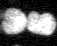
\includegraphics[width=\scalingfactor\textwidth]{images/joint/pipeline/78_raw_crop_enhanced.png}
        };
    \end{scope}
    \begin{scope}[every node/.append style={yslant=0.5,xslant=-1},yslant=0.5,xslant=-1]
        \begin{pgfonlayer}{bglower}
            \node[inner sep=0, label={[xshift=15]above:{}}] (raw2) {
                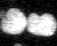
\includegraphics[width=\scalingfactor\textwidth]{images/joint/pipeline/79_raw_crop_enhanced.png}
            };
        \end{pgfonlayer}
    \end{scope}
    \coordinate (base1) at (raw2.north west |- raw2.south west);
    \coordinate (base2) at (raw2.south east |- raw2.south west);
    % \draw [pllbl]
    % (base1) -- (base2) node[black,midway,yshift=-0.6cm]
    % {Raw Data};
    \path let \p1 = (base1.west), \p2 = (base2.east) in
    node[pllbltxt, minimum width=\x2-\x1] (labelraw) at ($(base1)!0.5!(base2)$)
    {\phantom{g}Raw Data\phantom{g}};
    \begin{pgfonlayer}{bglower}
        \path[threed] (raw2.south east) -- (raw1.south east);
        \path[threed] (raw2.north east) -- (raw1.north east);
        \path[threed] (raw2.south west) -- (raw1.south west);
        \path[threed] (raw2.north west) -- (raw1.north west);
    \end{pgfonlayer}
\end{scope}

%%% Local Variables: 
%%% mode: latex
%%% TeX-master: "../../../main"
%%% End: 
